\section{Implementation}

Our MLCache prototype was built on top of the Linux kernel version 4.14.0-rc7.
In this section, we provide a brief background to the page cache implementation
on Linux and describe how we modified it in order to add the learning model
described in Section~\ref{section:learning}.

\subsection{The Linux Page Cache}

Linux employs a modified version of the traditional LRU strategy called
\emph{two-list LRU}. As the name suggests, two LRU lists are maintained in this
approach: the \emph{active} and \emph{inactive} list. The active list contains
pages that have been accessed more than once in the past, whereas the inactive
list holds the set of pages that have been accessed only once. In other words,
the active list attempts to capture \emph{frequency} and the inactive list
represents \emph{recency}.

The following subsections introduce the main concepts that are relevant to our
work on MLCache. Figure~\ref{fig:lru} describes the two-list approach used in Linux.

\begin{figure}[h]
  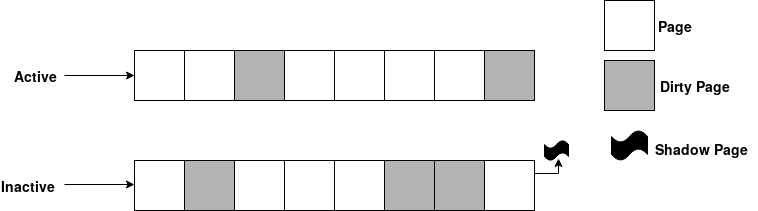
\includegraphics[scale=0.3]{img/LinuxLRU.png}
  \caption{The two-list LRU page cache on Linux. When a page is evicted (last
  page of the inactive list), it is replaced by a shadow page.}
  \label{fig:lru}
\end{figure}

\subsubsection{Dirty Pages}

As mentioned previously, the page cache holds blocks of data stored in the disk
device.  When user space applications perform write operations to certain
blocks of data, the corresponding pages are marked \emph{dirty}. Dirty pages
contain data that has not yet been flushed to the persistence device. In Linux,
dirty pages are not immediately flushed to the disk when the write operation
occurs; instead, the kernel periodically schedules a \emph{ writeback thread}
that scans the LRU lists and writes dirty pages to the disk.

\subsubsection{Cache Eviction}

When pages are read from or written to the disk, new entries are added to the
page cache.  As long as there is enough memory on the system, the number of
pages will keep growing, up to a certain threshold\footnote{Even a special
webpage was \cite{lamr} created in order to clarify this behavior, which
probably scares unfamiliar users.}. When the system is under memory pressure,
the kernel will create separate threads that will \emph{shrink} the LRU lists.
In particular, pages at the tail of the inactive LRU list are removed (pages
are always added to the head of an LRU list.) For this reason, Linux also
periodically ensures that the active and inactive lists are balanced: for
example, if too many pages are in the active list, the ones at the tail will be
demoted to the inactive list.

\subsubsection{Page Lookup}

Every page I/O operation on Linux goes through the page cache --- if the an
entry is found (\emph{cache hit}), an expensive call to the disk driver is
saved. Since these page lookups happen very often, they need to take a very
short time to produce a result. Linux 2.6 introduced a new page cache lookup
algorithm using \emph{radix trees} (as opposed to the old, global hash table in
previous kernels.) Each file contains its own radix tree of pages, and lookups
happen by providing only a file offset. Figure~\ref{fig:radix} illustrates the
radix tree approach, as defined in Linux 4.14.0-rc7.

\begin{figure}[h]
  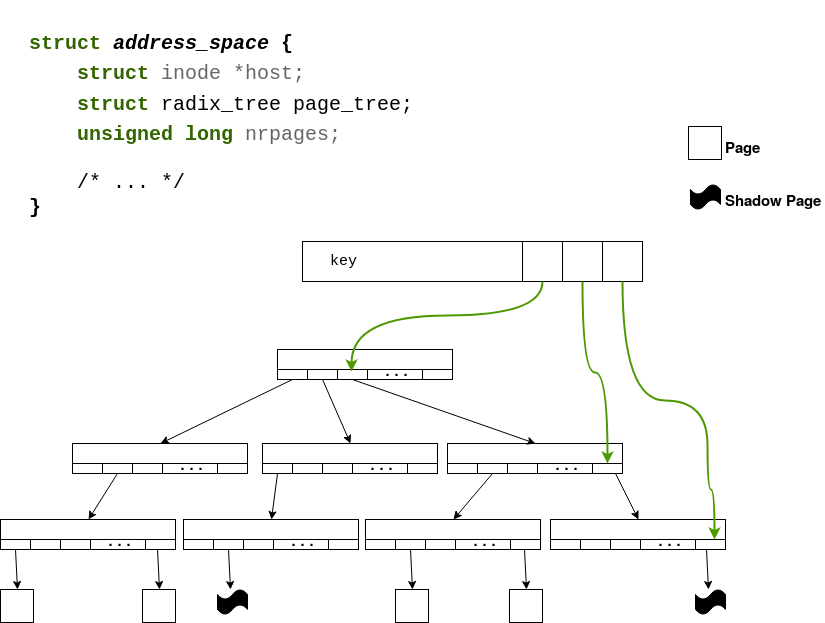
\includegraphics[scale=0.3]{img/LinuxRadixTree.png}
  \caption{The Linux page tree. Each file is represented by a (poorly named)
  \texttt{struct address\_space}, and contains a radix tree with pointers to
  locations where pages are kept in memory. When a page is evicted, a shadow
  page is placed in its previous spot. In the example lookup of this figure,
  \texttt{key} resolves to an entry with a shadow page. The corresponding page
  will likely be loaded directly into the \emph{active} LRU list.}
  \label{fig:radix}
\end{figure}

\subsubsection{Shadow Pages}

Another important optimization employed by the Linux page cache implementation
is the use of \emph{shadow pages}. Whenever a page is evicted, a special entry
--- called shadow page --- is created and replaces the spot previously occupied
by the recently evicted page in the radix tree. When a page lookup occurs and a
shadow page is found at the requested offset, the new page is added to the page
cache and inserted directly into the active LRU list. The use of shadow pages
is a cheap optimization (the shadow page is 16 bytes long, whereas a page is 4 KB
in x86) that can potentially avoid workflows that would cause thrashing.
